%!TEX root = ../../Main.tex
\graphicspath{{Chapters/Indledning/}}
%-------------------------------------------------------------------------------

\chapter{Shrinkage And Dimension Reduction Methods }
Contrary to subset selection methods, which uses least squares to fit a linear model containing a subset with \emph{n} of all \emph{p} predictors, shrinkage methods fits a model containing all \emph{p} predictors. This is done by a penalty that regularizes the coefficient estimates and thereby shrinks them towards zero. By shrinking the coefficient estimates their variance can be significantly reduced. In this section the two shrinkage methods Ridge regression and The Lasso will be covered.\\
Both shrinking methods tries to control variance by either using a subset of the original variables or by shrinking their coefficients towards zero and uses all of the original predictors. Another class of approaches, dimension reduction, is one that transforms the predictors first and then fits a least squares model using the transformed predictors. The reduction comes from the fact that the methods reduces the problem of estimating \(p+1\) coefficients to estimating \(M+1\) where \(M < p\). In this section the two dimension reduction methods Principal Component Regression and Partial Least Squares will be covered.


\section{Ridge regression}
Ridge regression is very similar to least square fitting in that it seeks to minimize RSS, but it adds a second term called the shrinkage penalty.\\ 
The equation \ref{ridge_regression_eq} shows the full equation for ridge regression. Here the first term is the RSS where \(\beta_0,...,\beta_p\) is to be estimated such that it is minimized, but the second term introduces a penalty to \(\beta_j\) which effectively shrinks it towards zero. This penalty is scaled with \(\lambda\) such that as it moves towards zero, the penalty moves towards zero and the equation produces the least squares estimates. Moving the tuning parameter towards infinity will in turn drive the coefficient estimates towards zero.\\ 
Thus ridge regression will produce a different set of coefficient estimates, \(\hat{\beta}_{\lambda}^{R}\), for each value of \(\lambda\) hence making it a tuning parameter. It is then critical to choose a good value for \(\lambda\), which can be done e.g. by the cross-validation method.

\begin{equation}
\sum_{i=1}^{n}(y_i - \beta_0 - \sum_{j=1}^{p}\beta_jx_ij)^2 + \lambda\sum_{j=1}^{p}\beta_{j}^{2}\label{ridge_regression_eq}
\end{equation}

The advantage of ridge regression over standard least squares comes from the bias-variance trade-off. By increasing the value of \(\lambda\) and thereby the effect of the penalty term, it is possible to decrease the variance of the predictor however the bias increases. As the test MSE (mean squared error) is a function of the variance plus the squared bias, finding a \(\lambda\) value which decreases the variance more than it increases the bias can result in a lower test MSE. Thus ridge regression will be superior whenever the least squares estimates have high variance.

\section{The Lasso}
The Lasso improves upon a disadvantage of ridge regression, namely that it includes all \emph{p} predictors in the final model, because it only reduces the magnitudes of the coefficients but never actually excludes any of them. Where ridge regression uses the \(\ell_2\)-norm in its regularization term (equation \ref{ridge_regression_eq}) , the Lasso uses \(\ell_1\)-norm (equation \ref{the_lasso_eq}). This has the effect of forcing some of the coefficients to be zero, depending on te value of \(\lambda\), instead of only driving them towards zero. Therefore the Lasso acts like subset selection, as it effectively performs variable selection yielding a sparse model which exactly is its improvement over ridge regression.\\
Selecting a good value for \(\lambda\) is critical just as it is for ridge regression and can be done by cross-validation.

\begin{equation}
\sum_{i=1}^{n}(y_i - \beta_0 - \sum_{j=1}^{p}\beta_jx_ij)^2 + \lambda\sum_{j=1}^{p}|\beta_{j}|\label{the_lasso_eq}
\end{equation}


\section{Principal Component Regression}
As with all dimension reduction methods Principal Component Regression (PCR) works in two steps: first transformed predictors are obtained and then a model is fit using the transformed predictors.\\
The underlying method for obtaining the transformed predictors is in this case PCA (Principal Component Analysis).
PCA derives a low-dimensional set of features from a large set of variables by acquiring basis vectors, \emph{principal components}, that forms an orthogonal basis. This is done by finding vectors with values that minimizes the sum of squared perpendicular distances between each point and the vector. Finding the next principal component is done as a linear combination of the variables that is uncorrelated with the principal component before it and has the largest variance. Up to \(M <= p\) principal components can be constructed this way, with \emph{p} being the number of predictors. By this construction the first principal component will contain the most information of the data-set with each following principal component containing less and less information.\\
Fitting a least square model to \(Z_1,...,Z_M\) principal components instead of \(X_1,...,X_p\) data points with \(p << M\), can in theory lead to better results as it can mitigate overfitting. This stems from the notion that most or all of the information in the data relating to the response if contained in the \(Z_1,...,Z_M\) principal component. If however \(p == M\) PCR will perform the same as doing least square fitting on all of the original predictors.\\
In PCR the number of principal components \emph{M} used for least square fitting becomes a hyper parameter that needs to be chosen carefully. This is typically done using the cross-validation method.


\section{Partial Least Squares}
In PCR the M principal components is guaranteed to best explain the predictors, however they are not guaranteed to best explain the response. This is due to the unsupervised nature of PCR, where the response does not supervise the identification of the transformed features (principal components).\\
Unlike PCR, Partial Least Squares (PLS) is supervised in the sense that the response is used to identify the transformed features that not only approximates the original predictors but also relates to the response.\\
PLS first identifies a new set of features \(Z_1,...,Z_M\) that represents \(M < p\) linear combinations of the original \emph{p} predictors. This is done by first standardizing the \emph{p} predictors. Then the first translated feature \(Z_1\) is calculated as in equation \ref{linear_combination_eq}, with the difference that each \(\theta_{j1}\) is set equal to the coefficient from the simple linear regression of the response \emph{Y} onto \(X_j\). In doing this tweaked version PLS places a higher weight on variables that are strongly related to the response. To compute \(Z_2\) the residuals from regressing each variable on \(Z_1\) are then used following the same calculations as for determining \(Z_1\). Lastly least squares as in equation \ref{transformed_linear_regression_eq} is used to fit a linear model to predict Y using \(Z_1,...,Z_M\) translated feature instead of the original \emph{p} features just like in PCR.

\begin{equation}
Z_m = \sum_{j=1}^{p}\phi_{jm}X_j\label{linear_combination_eq}
\end{equation}

\begin{equation}
y_i = \theta_0 + \sum_{m=1}^{M}\theta_{m}Z_{im} + \epsilon_i\label{transformed_linear_regression_eq}
\end{equation}

\section{Lab results}

Principal Component Regression(PCR) and Partial Least Squares(PLS) has been applied on the data set "Hitters" to predict salary as in exercise 6.7.1 and 6.7.2 in the course book. This has been done by finding the number of components that gives the smallest MSE on the training set.\\
Tenfold cross validation has been used to find the MSE as a function of components as seen on code listing \ref{lst:MSE_PCR} showing the implementation for PCR. A similar implementation has been used for PLS. The cross validation has been done for 10 components, as PCA shows an explained variance of over 90\% with a flattened curve beyond 10 components, as seen on figure \ref{fig:PCA_hitters_dataset}.\\
The results for PCR can be seen on figure \ref{fig:MSE_PCR}, where six principal components gives the lowest MSE. For PLS the lowest MSE value is achieved using only two components.
Applying PCR with seven components on the test set gives a MSE of 114098.06, while applying PLS with two components on the test set gives a MSE of 104838.51. Thus for the data set used in this example PLS clearly performs better with both a lower component count and a lower MSE value on the test set.

\begin{lstlisting}[language=Python, caption=Code snippet showing tenfold cross validation of PCR]
def subset_Process(predictor, X, y):	
	# Scale the data
	pca = PCA()
	X_reduced = pca.fit_transform(scale(X_train))	
	# Setup folds and linear regression
	mse = []
	regr = linear_model.LinearRegression()
	kf_10 = KFold(n_splits=10, shuffle=True, random_state=1)
	# Single CV to get MSE for the intercept
	score = cross_val_score(regr, np.ones((len(X_reduced),1)), y.ravel(), cv=kf_10, scoring='neg_mean_squared_error').mean()    
	mse.append(-score)
	# CV for pc principal components
	for i in np.arange(1, pc):
		score = cross_val_score(regr, X_reduced[:,:i], y, cv=kf_10, scoring='neg_mean_squared_error').mean()
		mse.append(-score)
	# Plot MSE as function of principal components after linear regression
	....
\end{lstlisting}\label{lst:MSE_PCR}

\begin{figure}[H]
	\centering
	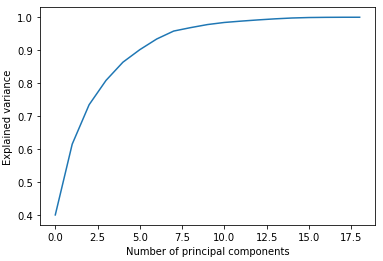
\includegraphics[width=7cm]{Img/PCA_hitters_dataset.PNG}
	\caption{PCA on the dataset "Hitters"}
	\label{fig:PCA_hitters_dataset}
\end{figure} 

\begin{figure}[H]
	\centering
	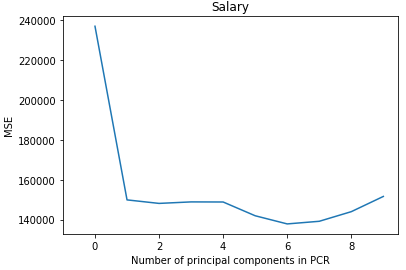
\includegraphics[width=7cm]{Img/MSE_PCR.PNG}
	\caption{MSE as a function of components in PCR}
	\label{fig:MSE_PCR}
\end{figure} 

\begin{figure}[H]
	\centering
	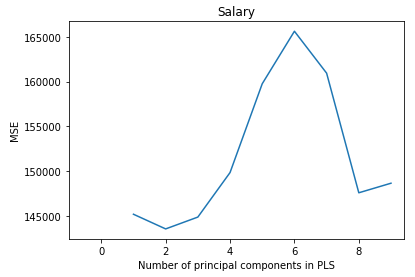
\includegraphics[width=7cm]{Img/MSE_PLS.PNG}
	\caption{MSE as a function of components in PLS}
	\label{fig:MSE_PLS}
\end{figure} 